\chapter{Introduction and Motivation}

\section{Phytoplankton and the Red Sea Ecology: Significance, Large-Scale
Features, and Applications}

\subsection{The Importance of Phytoplankton}

Phytoplankton are unicellular, free-floating, photosynthetic algae that live in
the upper layers of bodies of water (ocean, lakes, rivers or ponds). There
exists a wide diversity of phytoplankton species. Up to date, about 5000 of
them have been identified \citep{Tett1995}. Phytoplankton are also highly
variable in sizes, ranging from \SI{0.2}{\micro\metre} for cyanobacteria to
\SI{200}{\micro\metre} for the largest species of diatom \citep{Pal2014}. In
the oceans, phytoplankton live in the surface layer where there is enough
sunlight for photosynthesis. 

Phytoplankton play a fundamental role for the ocean ecology. They are at the
basis of the marine food web and trap most of the energy used by pelagic
ecosystems \citep{Pal2014}. Zooplankton graze phytoplankton, which are in turn
consumed by higher trophic levels. It has been estimated that nearly 98\% of
the ocean primary productivity comes from phytoplankton \citep{Pal2014}.
Phytoplankton are also responsible for maintaining the dissolved oxygen level
necessary for other species to survive \citep{Pal2014}.  However, high
phytoplankton concentration may also impact their environment by creating dead
zones. When they die and sink, the bacteria that decompose them can consume all
the available oxygen \citep{Pal2014}, and this may cause massive mortality in
the fauna. Moreover, because of its short life cycle, phytoplankton respond
very well to changes in its environment, making it a key parameter to monitor
water quality \citep{Wu2014}.

Phytoplankton place at the bottom of the marine food chain makes it an
important factor for fisheries. Productive fishing zones such as the regions in
the Arabian seas, Californian coast, north-west African coast and Chilean
coast, are due to the upwelling of cold nutrient rich water favourable to
phytoplankton growth \citep{Mann2006}.
As such, remotely-sensed chlorophyll data have been
routinely used since the last decade to help fisheries predict the timing of
phytoplankton blooms \citep{Robinson2010}. The El-Nino phenomenon is known to
create less favourable conditions for phytoplankton in the Eastern Pacific,
resulting in a dramatic reduction of fish catches of fisheries in the western
coast of South America \citep{Robinson2010}. In contrast, in the Red Sea, the
MEI (Multivariate ENSO Index) has been found to positively correlate with
chlorophyll concentration, which may have a important implications for regional
fisheries \citep{Raitsos2015}.

Phytoplankton also plays the role of a biological CO2 pump and strongly impact
the Earth climate. During photosynthesis, phytoplankton captures carbon and
releases oxygen. A part of this organic material stays in the food web, either
transmitted to higher trophic level, or degraded  by bacteria. Another part
sinks to the bottom of the ocean to form sediments. It is estimated that
phytoplankton accounts for 48\% of Earth carbon fixation \citep{Pal2014}.

\subsection{Red Sea Large-Scale Phytoplankton Dynamics}

Typical tropical seas (TTS), such as the Red Sea, are characterized by a highly
stratified structure, where warm nutrient-depleted surface water is separated
from the cold nutrient-rich deep water by a steep gradient of temperature zone
called pycnocline. The pycnocline acts as barrier that limits the upward
nutrients flow \citep{Mann2006}. As a result, TTS are oligotrophic exhibiting
low chlorophyll concentrations. Until recently, marine biologists believed that
tropical and subtropical seas should have low productivity. However, recent
investigations have contested this idea, suggesting that different upwelling
mechanisms (winter deep mixing, storms, eddies, etc) occur in these regions,
and bring new nutrients to the surface water \citep{Mann2006}.

Despite being an oligotrophic and challenging environment for marine life, the
Red Sea has a surprisingly rich and diverse ecosystem \citep{Raitsos2011},
and a very well developed coral reef system \citep{Racault}. The source of
nutrient for sustaining such a developed ecosystem is not well understood yet,
but the exchange with the open ocean, the atmospheric depositions and transport
through the mesoscale eddies are believed to be major factors.
\citep{Raitsos2013, Zhan2014}.

Although the Red Sea environment is still relatively well preserved, it is
increasingly stressed by human activities. The continuous urbanization and
fishing activity contribute to the fragilization of this unique ecosystem
\citep{Acker2008}. An abrupt increase of temperature has further occurred in
the last decade, which may further threaten its fragile coral reef system
\citep{Raitsos2011}.

Because of the lack of in-situ measurements, the large-scale phytoplankton
dynamics of the Red Sea remain largely unknown \citep{Raitsos2013,
Triantafyllou2014}. In very recent studies, remotely-sensed data and computer
simulations have been used to improve our knowledge of the ecology of this
region. The Red Sea is deficient in major nutrients \citep{Weikert1987}, and
the only significant input of nutrient-rich water comes from the Gulf of Aden
\citep{Yao2015}. This explains the general pattern of chlorophyll concentration
increase from north to south \citep{Raitsos2013}, with the lowest concentration
found in the northern central Red Sea, as can be seen in Figure \ref{meanchl}.
The Red Sea also displays a distinct seasonality, with a peak in concentration
during winter.  A weak summer peak is also observed over the whole Red Sea
around July, except in the northernmost region \citep{Raitsos2013}. Despite
this regularity, a strong interannual variability was observed, with blooms
that can reach mesotrophic concentration levels \citep{Raitsos2013}. According
to \citet{Triantafyllou2014}, the variations in the Red Sea ecology are mainly
driven by physical circulation. In the rest of this section, we explore some of
the mechanisms that have been linked to the major features of chlorophyll
concentration in the Red Sea.

\begin{figure}[h]
    \centering
    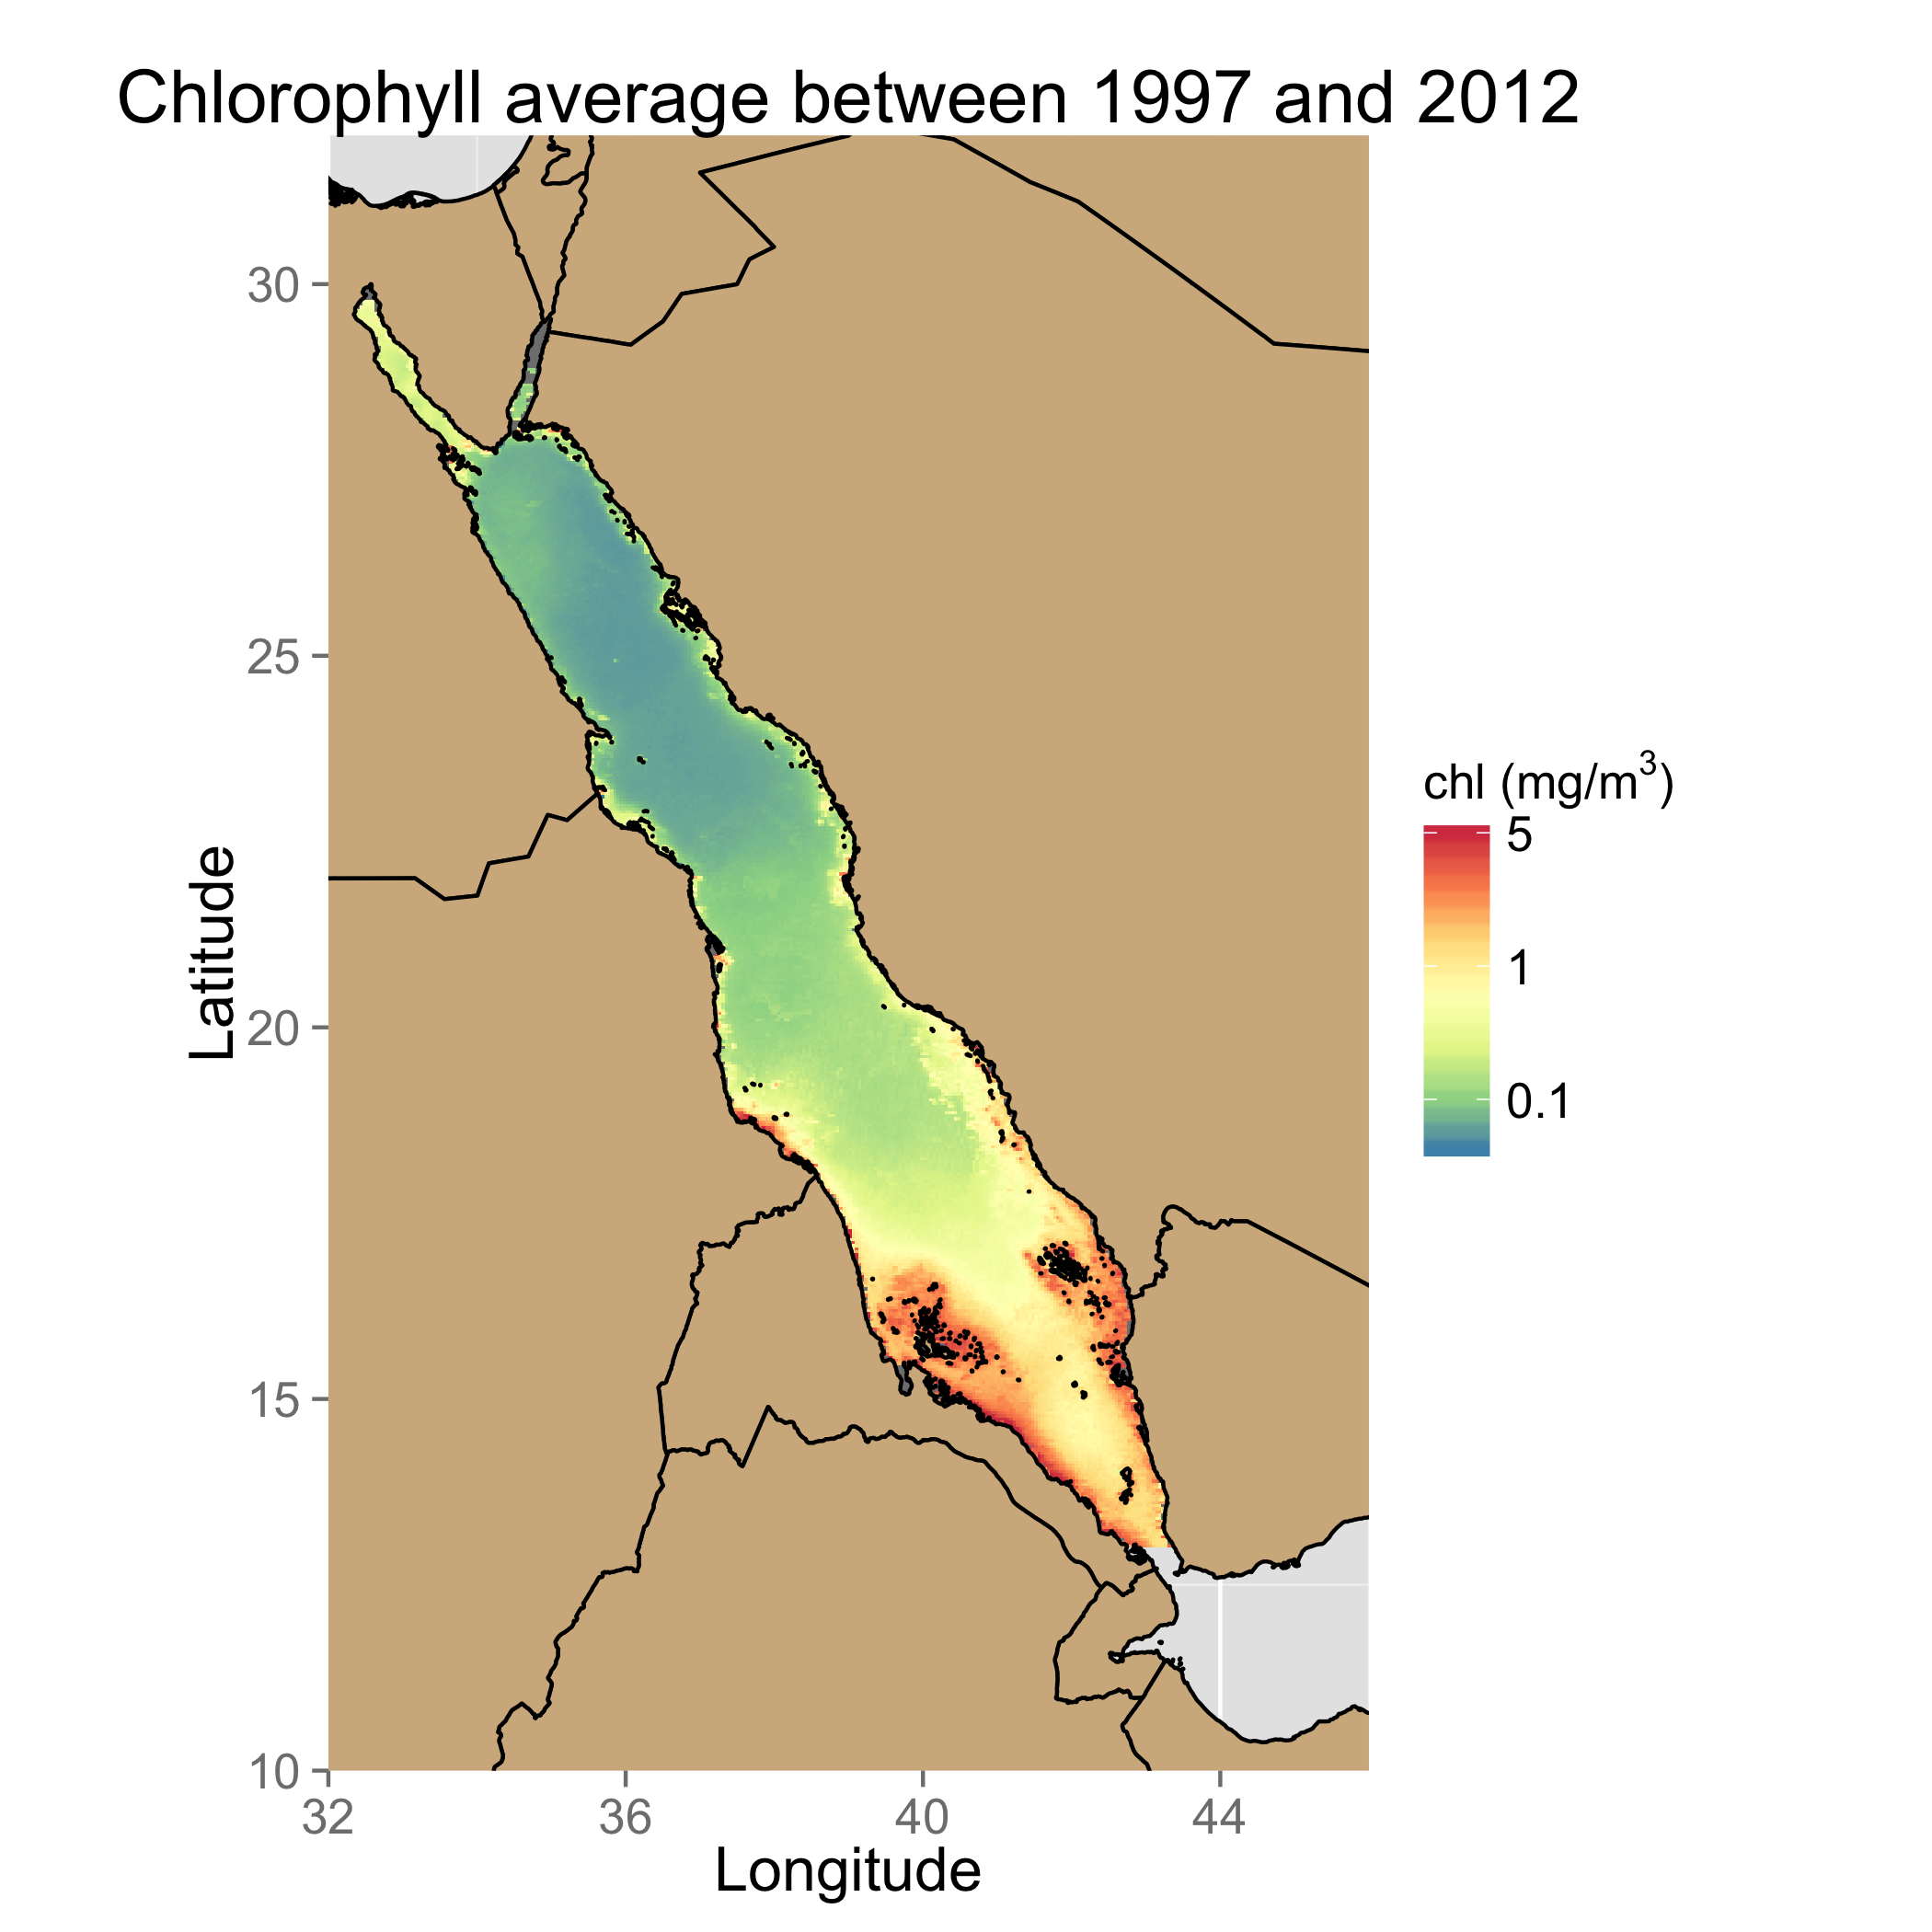
\includegraphics[scale=.15]{figures/chl_average.png}
    \caption{Average chlorophyll concentration from CCI data}
    \label{meanchl}
\end{figure}

The exchange of water with the nutrient-rich Gulf of Aden is a major driving
mechanism of the Red Sea productivity \citep{Triantafyllou2014}. It is believed
to be the most important source of nutrients. The maximum chlorophyll
concentration observed in the southern Red Sea during winter is attributed to
wind-driven water intrusion \citep{Raitsos2013, Yao2014}. In Summer, this
exchange of water is believed to be the major source of nutrients for the whole
Red Sea. The influence of the water intrusion weakens as the latitude
increases, explaining the low concentration in the northern half of the Red Sea
\citep{Raitsos2013}.

Deep convection also plays an important role in allowing nutrient-rich deep
water to mix with water of the euphotic zone. Vertical mixing is the most
vigorous in the northern extremity of the Red Sea during winter. This
explains its higher chlorophyll concentration compared to the north-central Red
Sea, a region of weak mixing \citep{Raitsos2013}. The northern Red Sea mixing
is believed to be mainly driven by wind \citep{Raitsos2013}.

The Red Sea circulation is strongly influenced by mesoscale eddies
\citep{Yao2014, Yao2014b, Zhan2014} that could impact primary production
\citep{Zhai2013}. In particular, the anti-cyclonic eddy in the central Red Sea
is believed to drive the June concentration peak and the summer productivity
of this region, by transporting nutrients and/or phytoplankton from the
adjacent coral reefs \citep{Raitsos2013}. In the northern Red Sea, a cold-core
eddy plays a role in enhancing the vertical mixing in this region
\citep{Raitsos2013}.

Aerial depositions of dust could also be an important input of nutrients for
the Red Sea, but it has been largely left unexplored \citep{Triantafyllou2014}.
\citet{Raitsos2013} noticed for example that sand storms in the Red Sea most
frequently happen in June and July, which coincides with the summer chlorophyll
peak. Finally, climate mode indices have been shown to be strongly correlated
with air-sea heat exchanges in the Red Sea \citep{Abualnaja2015}, and might
therefore influence its biology. This has been recently confirmed by
\citet{Raitsos2015}, who have shown that El Nino has a positive impact on the
chlorophyll concentration, by strenghtening the wind transporting nutrients
into the Red Sea from the Gulf of Aden.

\section{Remotely-Sensed Chlorophyll Data: Relevance and Challenges for the Red
Sea}

\subsection{Measuring Chlorophyll Concentration}

Chlorophyll is a molecule present in algae, phytoplankton and plants that is
critical for photosynthesis. It is a poor absorber of green light, and is
responsible for the coloration of plants \citep{Pal2014}. When phytoplankton
are present in high concentrations, the water usually takes a detectable green
coloration (it may also take a red or blue coloration depending on the type of
dominating phytoplankton) \citep{Robinson2010}. This offers an efficient way to
monitor the phytoplankton concentration from space.

In-situ measurement of chlorophyll concentration can be gathered through
scientific cruises, buoy stations or gliders (unmanned submarines). These
methods are expensive to deploy and therefore generally have limited temporal
and spatial coverage \citep{Robinson2010}. Political issues, as in the Red Sea,
as well as security issues, as in the Arabian Sea, set also barriers to in-situ
measurements.

Satellite measurements of chlorophyll provide excellent proxies for
phytoplankton concentrations with a good temporal and spatial coverage
\citep{Robinson2010}. The SeaWIFS, MODIS and MERIS missions have provided an
uninterrupted coverage of global ocean since 1997. High-resolution maps of
daily chlorophyll concentration are freely accessible to the scientific
community \citep{McClain2009}. Despite some limitations, such as missing data
due to cloud coverage and sunglint, or problematic values in coastal areas,
remotely-sensed chlorophyll concentrations are intensively used by the
scientific community. In regions, like in the Red Sea, where little in-situ
measurements are available, these constitute the most important data source
\citep{Raitsos2013, Brewin2013}.

\subsection{Limitation of Remotely-Sensed Chlorophyll Data in the Red Sea}

The quality of remotely-sensed chlorophyll data products such as MODIS and
SeaWiFS in the Red Sea is comparable with that of the rest of the world for
case I waters (open sea) \citep{Brewin2013}. However, the data contains a large
amount of missing values because of persistent clouds, sun-glint and sensor
saturation \citep{Racault}. This problem is particularly acute during the
summer in the southern Red Sea where the data coverage is almost null
\citep{Racault}, as shown in Figure \ref{misval_modis}.

Chlorophyll concentration estimation in optically complex case II waters is a
recurrent problem in this remotely-sensed data that particularly affects the
southern Red Sea.  In this region, the remotely sensed chlorophyll data could
be overestimated \citep{Raitsos2013}. However, all high values are not
necessarily wrong, as highly productive coral reefs are also present in this
region \citep{Raitsos2013}. These values have however not been validated yet,
because of the lack of in situ measurements \citep{Raitsos2013}.

\begin{figure}[h]
    \centering
    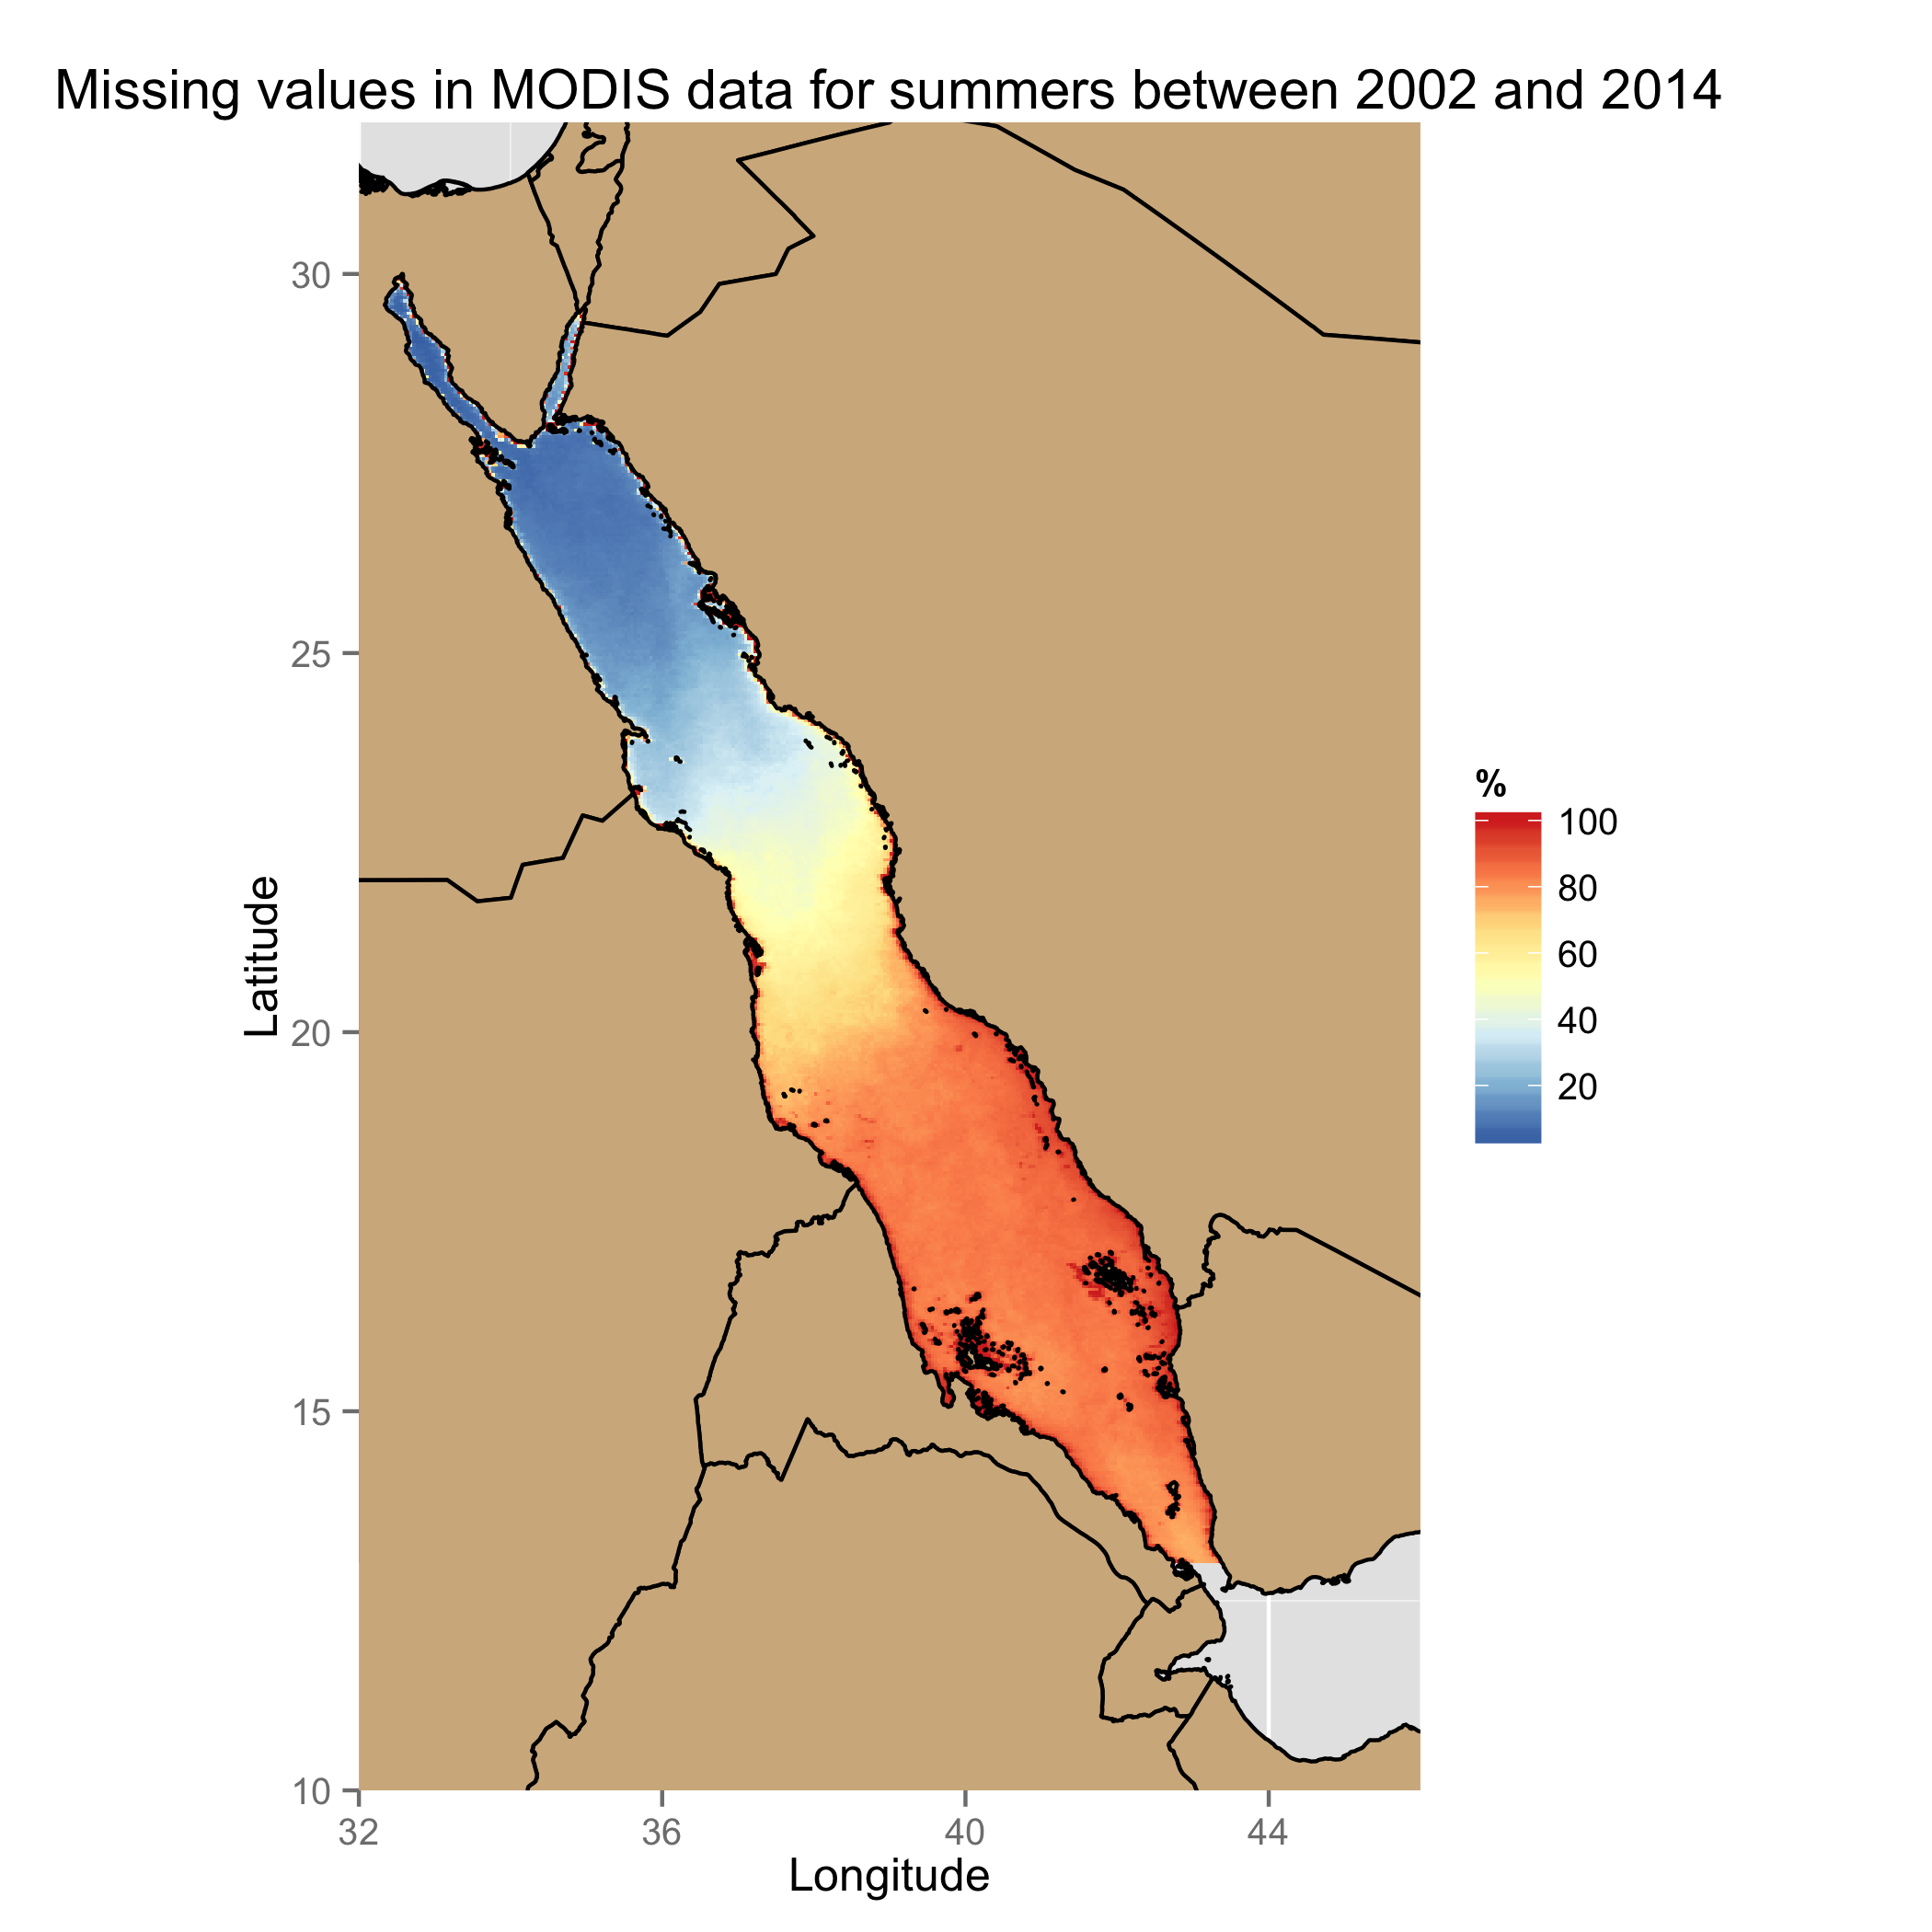
\includegraphics[scale=.15]{figures/modis_missing_values_summer.png}
    \caption{Percentage of missing values in the MODIS chlorophyll dataset}
    \label{misval_modis}
\end{figure}

One solution to missing and bad values is to apply a data filling algorithm, of
which one of the most popular algorithm is the Date INterpolating Empirical
Orthogonal Functions (DINEOF), which is an EOF based data filling approach
introduced by \citet{Beckers2003}. In \citet{Sicarjobs2011}, it has been
employed to fill chlorophyll data with 70\% of missing values.
\citet{Taylor2013} compared DINEOF with other EOF-based reconstruction
algorithms, suggesting that the former is a better method for data filling.
DINEOF has been further employed in several other chlorophyll studies
\citep{Miles2010, Waite2013}, and has also been used for multivariate
reconstruction of SST fields using chlorophyll data in \citet{Alvera2007}. 

The OC-CCI is a new chlorophyll data product that considerably increases the
Red Sea coverage. It is a merged product from the SeaWiFS, MODIS and MERIS data
missions.  Overall, it achieves a 75-80\% coverage in the entire Red Sea basin
against 50-65\% for a single sensor \citep{Racault}. During the summer, the
improvement in coverage is dramatic, as shown in Figure \ref{misval_cci}.
This is mostly
due to the use of the POLYMER algorithm \citep{Steinmetz2011} that allows to
exploit MERIS data collected during hazy conditions. This new dataset
has not been fully studied to revisit the assumptions made on the large-scale
Red Sea phytoplankton productivity.

\begin{figure}[h]
    \centering
    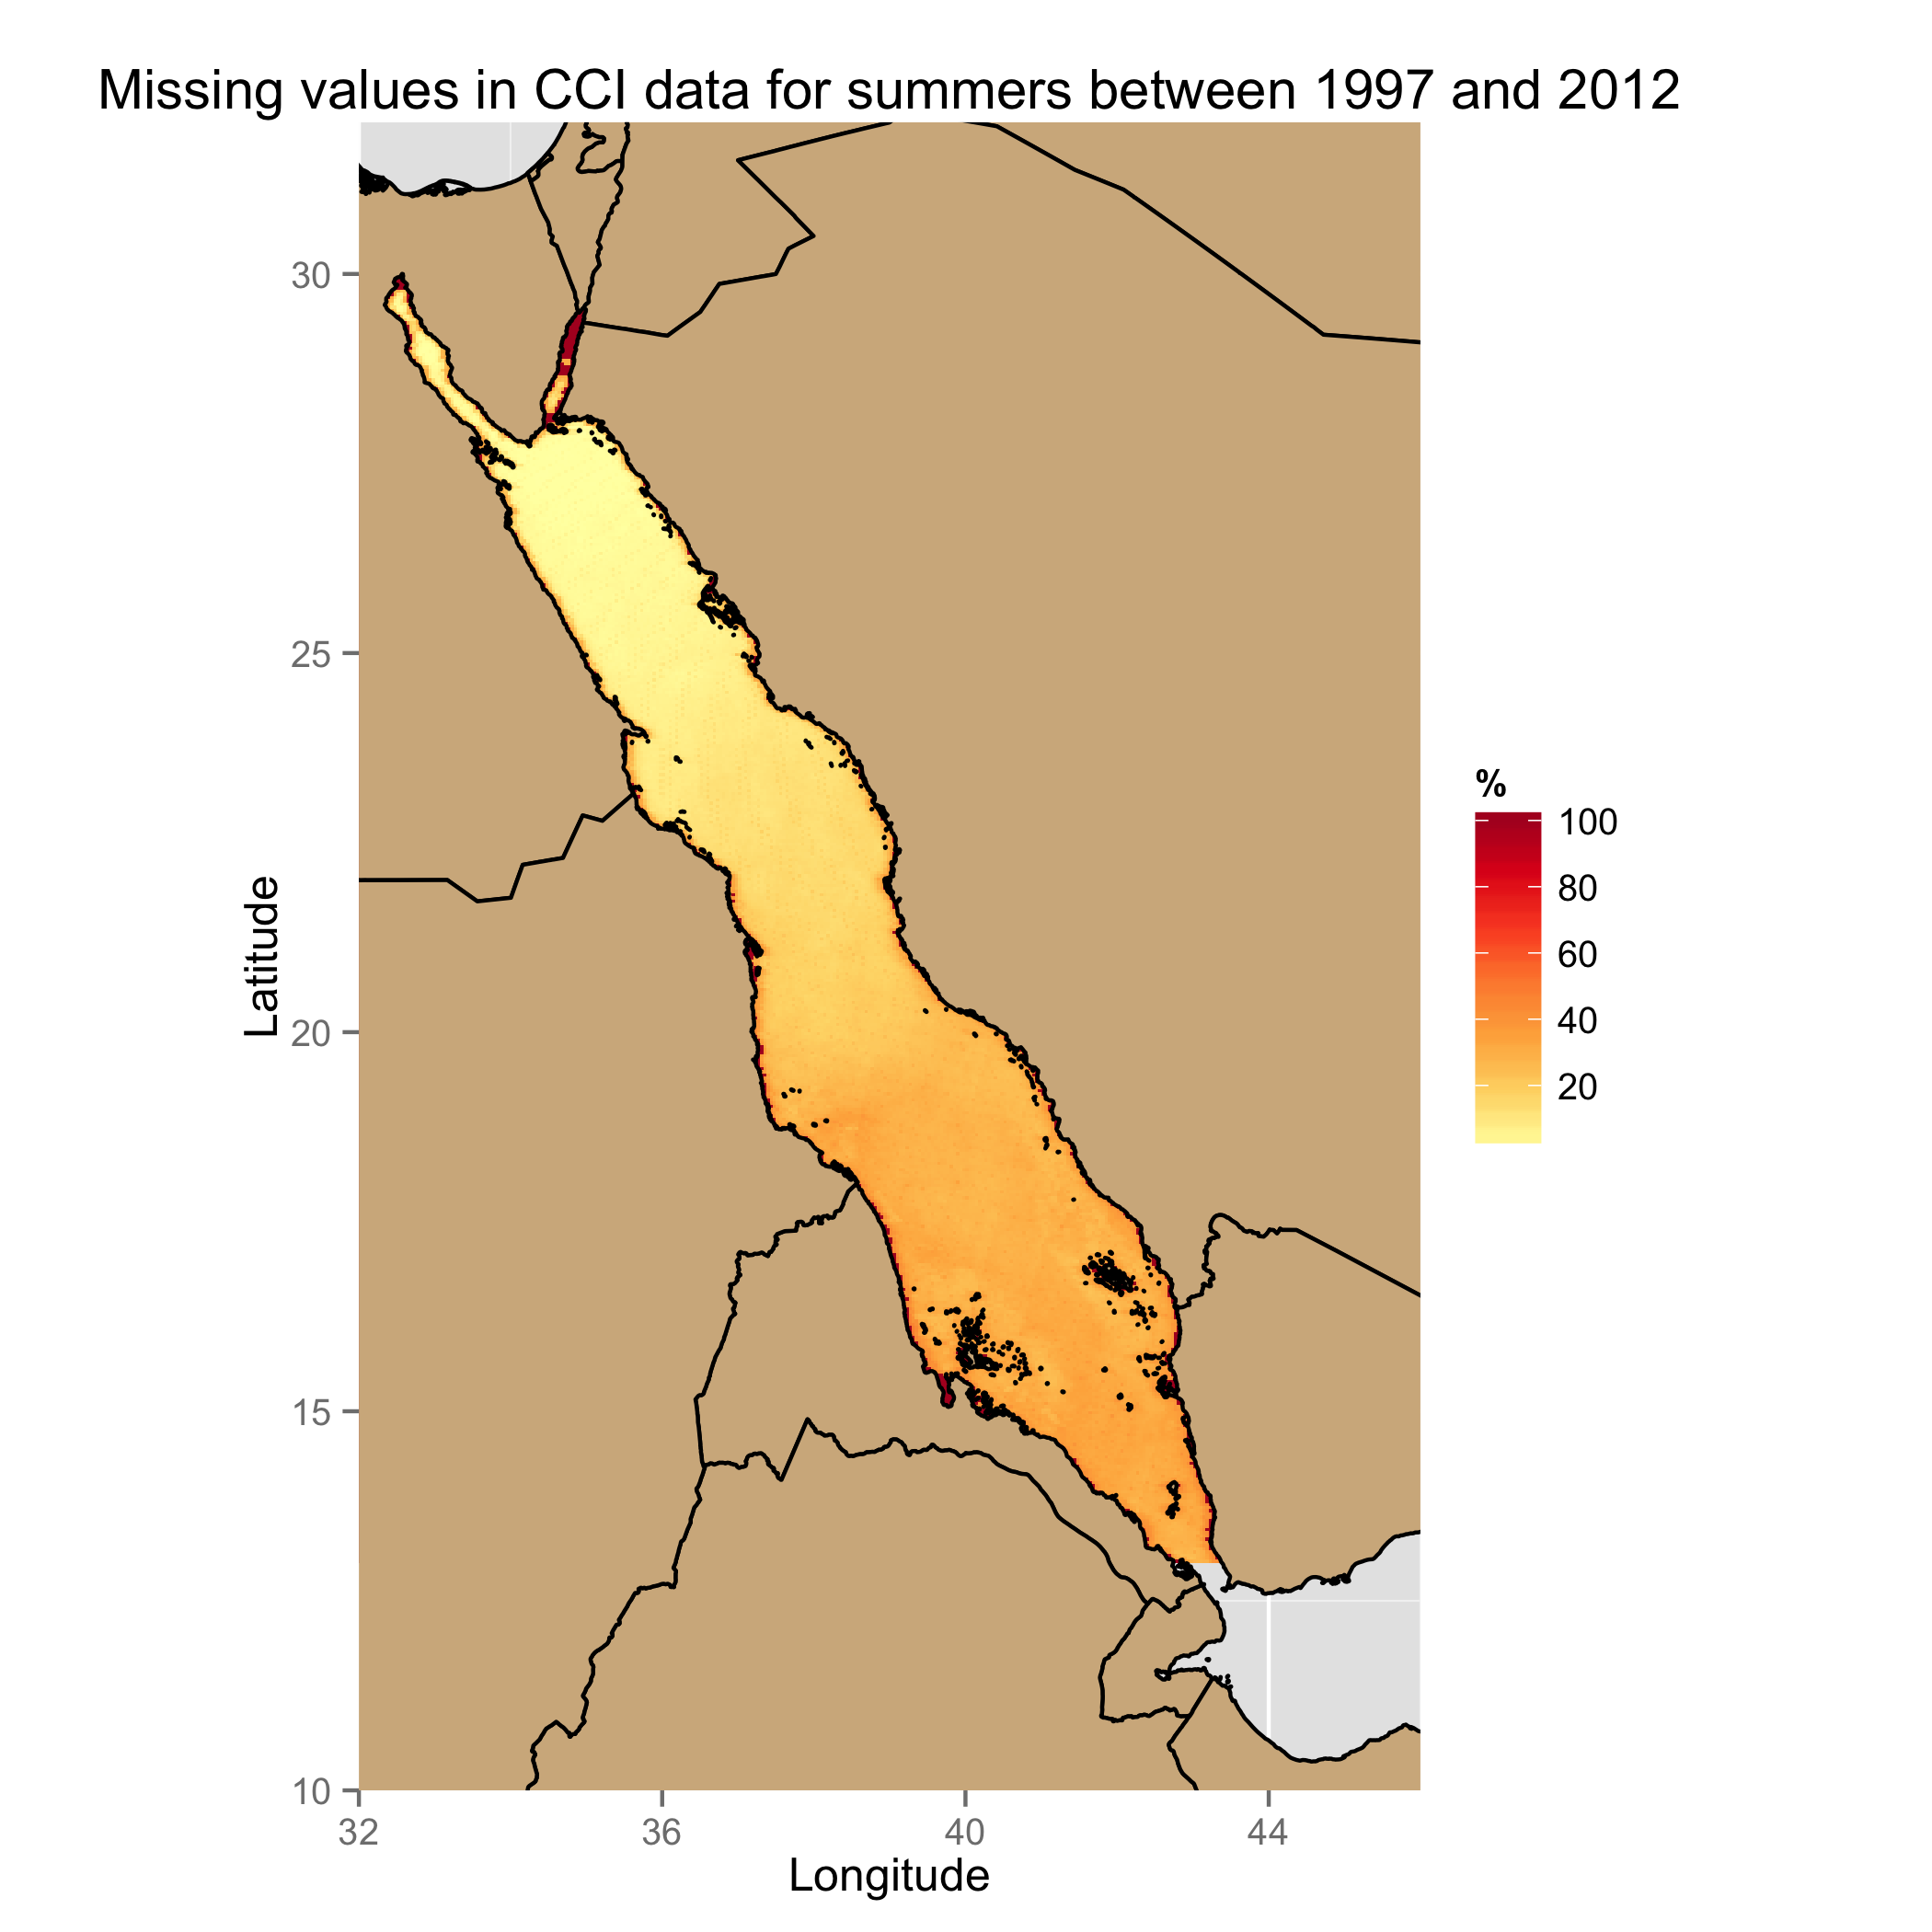
\includegraphics[scale=.15]{figures/cci_missing_values_summer.png}
    \caption{Percentage of missing values in the CCI chlorophyll dataset}
    \label{misval_cci}
\end{figure}

\section{Modeling and Forecasting Chlorophyll: Data and Dynamics Driven
Approaches, and Applications}

\subsection{Why Modeling Chlorophyll?}

Models could be useful to identify causes behind observed chlorophyll patterns.
Many hypotheses have been made about the drivers of chlorophyll concentration
in this regions, but some of them have not been yet investigated through
models. The role played by the exchange of water with the Gulf of Aden and
winter overturning in the northern Red Sea have been successfully modeled with
a 3D coupled physical-ecological model \citep{Yao2014, Yao2014b,
Triantafyllou2014}.  However, the interaction between the open sea and coral
reefs, and the role of atmospheric depositions have not been investigated yet.
Models, can also be helpful for understanding governing dynamics affecting the
chlorophyll concentration. In particular, the interaction between the
productivity level of the different regions of the Red Sea is yet to be
explored.

Model predictions of chlorophyll concentration also have practical applications
for fisheries. Furthermore, phytoplankton blooms can be harmful to humans and
marine life and are closely monitored in many regions of the world
\citep{Pettersson2013}. In the Red Sea, where tourism and aquaculture are
developing, it is likely to become a concern too. Phytoplankton is also
directly, and indirectly through zooplankton, the cause of microfouling that
affects desalination plants. In 2008-2009, a red tide forced the shutdown of
desalination plants along the Gulf of Oman and the Arabian Gulf
\citep{Richlen2010}.


\subsection{Deterministic Models}

\subsubsection{Ecological Models}

There is a rich literature on the modeling of marine ecosystems using
differential equations (see \citet{Fennel2004} for an introduction). In these
models the interactions of complex physical, chemical and biological processes
are modeled by differential equations that represent the flow of carbon,
nitrogen, phosphate and silicon. The biota is divided into trophic levels, and
can be further divided by feeding methods and size classes
\citep{Baretta1995, Triantafyllou2014}.

Ecological deterministic models vary widely in complexity depending on
the number of interactions represented.  They can be as
simple as the nutrient-phytoplankton-zooplankton (NPZ) model
\citep{Anderson2005} that only has three variables representing two trophic
levels and nitrate, or as complex as the European regional seas ecosystem model
(ERSEM) that has dozens of variables \citep{Baretta1995}. NPZ models are
extensively used because of their simplicity and capacity to model the the
large-scale features of marine ecosystems \citep{Anderson2005}.
ERSEM has recently been coupled to the MITgcm circulation
model used to simulate the Red Sea ecology \citep{Triantafyllou2014}. However
the complexity of these models makes them difficult to parametrize when not
enough data are available, which is usually the case in many marginal seas
\citep{Anderson2005}. Ecological models usually have large uncertainties due to
the imperfect modelization, the unknown initial conditions and the
uncertainties in the parametrization \citep{Edwards2015}.

\subsubsection{Data Assimilation}

Data assimilation is used to improve the simulations of ecological dynamical
models and enhance their forecasting capabilities by constraining their
predictions with available observations \cite{Edwards2015}. Such prediction
capabilities are deployed in operational expert systems, for example to study
the impact of human activities on the ecosystem of the Gulf of Pagasitikos
\citep{Korres2012}. The deployment of a similar forecasting system in the Red
Sea is currently under development \citep{Triantafyllou2014}. Hindcasting, the
estimation of unobserved variables, is another application of assimilation
systems. \citet{Ciavatta2011} showed that data assimilation of ocean color data
may improve the seasonal and annual hindcast of non-assimilated biogeochemical
properties in the shelf area of Western English Channel. Data assimilation can
also be used for reanalysis, to provide estimates of biogeochemical
distributions of the past \citep{Fontana2013}.

In the marine ecology modeling community, three assimilation schemes have been
widely used: the Ensemble Kalman filters (EnKF), the Singular Evolutive
Extended Kalman filter (SEEK), and its ensemble variant, the Singular Evolutive
Interpolated Kalman filter (SEIK). The stochastic EnKF, a Monte-Carlo
approximation of the Kalman Filter, has been used in \citet{Ciavatta2011,
Ciavatta2014}. This scheme may however suffer from sampling errors when the
ensemble size is smaller than the number of observations, as is usually the
case when assimilating remotely-sensed data \citep{Nerger2005, Altaf2014}.
SEEK is a reduced-rank variant of the Extended Kalman filter (EK). It was
introduced for efficient data assimilation into large scale ocean models.  It
is based  on the projection of the error covariance onto a low dimensional
space.  SEEK has a long history in data assimilation for marine ecology models
and is still extensively used in recent studies \citep{Fontana2013, Korres2012,
Butenschon2012}.  SEIK is an ensemble variant of the SEEK  and a deterministic
version of the EnKF that do not suffer from observations sampling errors, as it
updates the filter forecast exactly as in the Kalman filter. It therefore
requires a resampling step to generate a new analysis ensemble for the next
forecast step. SEIK has been used by \citet{Triantafyllou2013, Korres2012}.
\citet{Korres2012} shows that SEIK and SEEK are both comparably robust methods
for highly nonlinear systems. \citet{Hoteit2005} has shown that SEIK
outperforms SEEK when using a high-resolution nonlinear model.

Ecological models are challenging applications for state of the art data
assimilation schemes \citep{Edwards2015}. First, biogeochemical variables are
usually positive concentration, whereas Kalman filters expect Gaussian
variables, and log-transformation may fail to avoid this issue
\citep{Ciavatta2011}. In an attempt to mitigate this problem,
\citet{Fontana2013} introduced Gaussian anamorphosis transformations.
Second, ecological blooms are intermittent and highly nonlinear, conditions
that are challenging for Kalman filter-based assimilation schemes
\citep{Hoteit2005}. Third, SEIK, EnKF and SEEK project the
error covariance onto some subspace, resulting in an underestimation of the
estimation error. \citet{Butenschon2012} studied different ways to propagate
the error covariance in order to alleviate this issue. Finally, the model error
statistics are required by Kalman-derived filters, but are difficult to
estimate. \citet{Triantafyllou2013} proposed to use the $H_\infty$ method with
SEIK in order alleviate this requirement.

Particle filters represent a class of data assimilation schemes that, unlike
Kalman-based filters, do not require any linearity or Gaussianity assumption
\citep{Edwards2015}. As such, they might be more suitable for data assimilation
into ecosystem models. They have been studied in the case of 0D and 1D
ecological models \citep{Edwards2015}, but are still strongly limited by their
demanding computational requirements. Their application to 3D model is an
active field of research \citep{Edwards2015}.


\subsection{Data-Driven Approaches}

Compared to data assimilative ecological models, data-driven statistical models
are relatively simpler to develop. Such models are usually
relevant when the phenomenon
producing the data is dynamically complex to model, or simply poorly understood
\citep{Gareth2013}. Various data-driven models have been proposed
to predict chlorophyll
concentration, mostly in small regions with complex dynamics (see references
below). Some statistical models, such as linear regression, Gaussian additive
models, or tree regression have the advantage of being easy to interpret
\citep{Gareth2013}, and could be used to understand the dynamics driving the
chlorophyll concentration \citep{Raitsos2012}.

\subsubsection{Statistical Models}

Statistical and machine learning models have been recently used for estimation and
classification problems related to phytoplankton concentrations. One
application is the detection of harmful algal bloom from spatio-temporal
satellite dataset, that has been addressed by \citet{Gokaraju2011} in the Gulf
of Mexico using support vector machines. Another application is the estimation
of chlorophyll concentration in case II coastal water using satellite radiance
data. This problem has been considered by \citet{Kim2014} on the west coast of
South Korea, and by \citet{Camps-Valls2006} using a global dataset of in situ
measurements.  The former used the support vector regression algorithm, while
the latter used the random forest algorithm.

Machine learning algorithms, in particular Artificial Neural Networks,
are also very popular for forecasting regional chlorophyll concentration in regions
with very complex dynamics, where deterministic ecological models usually
perform poorly. Neural networks are also commonly used for forecasting
chlorophyll concentration in fresh as well as in coastal water systems. In
\citet{Jeong2006}, temporal recurrent recursive neural networks have been used
and found superior to traditional time-series models for daily forecasts of
chlorophyll concentration.  \citet{Wang2013} also used recurrent neural
networks for forecasting daily chlorophyll in Lake Taihu, China.
\citet{Mulia2013} combined Neural Network and genetic algorithm for nowcasting
and forecasting of the chlorophyll concentration up to 14 days ahead, in the
tidal dominated coast of Singapore.  Finally, \citet{Lee2003} used neural
networks for the forecasting of algal bloom with one or two weeks lags in the
coastal waters of Hong-Kong.

\subsubsection{Geostatistics}

Phenomena such as propagation and diffusion play a key role in the chlorophyll
spatial concentration, but are difficult to represent without spatial modeling.
There is also a difference in the chlorophyll patterns of different regions of
the Red Sea, in particular between the nutrient rich southern Red Sea and the
oligotrophic northern Red Sea, and between the open ocean and the coastal
waters \citep{Raitsos2013}.  One should also expect the different regions of
the Red Sea to interact.

In contrast to the statistical models presented above, in geostatistical
models, the spatial dimension is modeled explicitely by representing the data
as a spatial stochastic process \citep{Gneiting2007}. In classical
geostatistics, spatial data is modeled as the realization of a two- (or three-)
dimensional Gaussian process \citep{Gneiting2007}.  Geostatistics can be easily
extended to spatio-temporal datasets \citep{Gneiting2007}. Many ways for
constructing space-time covariance functions for these models have been
recently proposed \citep{Gneiting2002, Cressie1999, Stein2005}.

The theory of space-time geostatistics is closely related to that of spatial
statistics. In fact, the time dimension becomes an additional dimension. However,
the relationship between these two dimensions is derived from a dynamical process,
that must be taken into account in the definition of the covariance function
\citep{Gneiting2010}. Some space-time covariance models can actually be derived
from a physical formulation, such as the frozen fields \citep{Gneiting2010}, or
stochastic differential equations \citep{Brown2000, North2011}.

Physically-derived space-time covariance functions are not commonly used, and
the usual approach is to construct them from spatial and temporal covariance
functions \citep{Gneiting2010}. One of the most simple types are separable
covariance functions, that are the products of a spatial covariance function
and temporal covariance function. These are computationally efficient, but are
not suitable to represent space-time interactions \citep{Cressie1999,
Stein2005}, making them of limited use for modeling physical systems. The
Cressie, Huang spectral characterization theorem of space-time covariance
functions has opened the door to wider ways of constructing them. For example,
\citet{Gneiting2002} presented a simple criterion that allows their
construction from a very large class of models. 

Space-time geostatistical models have been used in a variety of applications.
\citet{Hohn1993} used it for forecasting the outbreaks of an invasive specie.
These methods have also been used in meteorology to model temperature fields
\citep{Handcock1994, North2011} or wind \citep{Cressie1999, Gneiting2002}, and
in environmental studies for ground-level ozone concentration. However,
they have not been applied to chlorophyll data.

\section{Thesis Objectives}

There is a crucial need for improving the modeling of large-scale features of
marine ecosystems. The ocean physical, chemical and ecological processes are
complex and poorly understood. Even though ocean color remote-sensing data has
revolutionized our understanding of marine ecology, it only gives information
about the phytoplankton at the sea surface. Our knowledge is even more limited
in the Red Sea, due to the paucity of in situ data.

The goal of this thesis is to develop novel models for efficient forecasting of
chlorophyll concentration in the Red Sea. Various methods will be developed and
tested following data and a dynamical-driven approaches. In particular, we will
develop efficient approaches to model the Red Sea chlorophyll, explore the
possibility of improving the state of the art data assimilative ecosystem
modeling, and introduce the use of geostatistics to the field of marine
ecology. The merits of both approaches will be compared for the first time in
the same region, and under the sames conditions. We will also propose ways to
efficiently combine both approaches methods for best forecasting of chlorophyll
concentration.

Currently, both deterministic and statistical approaches have been used to
predict chlorophyll. However, these approaches have never been compared, nor
combined in the same problem. A thorough comparison is very much needed. It
would provide modelers with a comprehensive foundation for developing their
modeling strategy. Combining them may further improve the forecasting skills.

This thesis will also help increase our understanding of the Red Sea ecology.
In particular, it will identify possibles drivers for the chlorophyll
seasonality and interannual variability. We will also identify and characterize
the different Red Sea eco-regions. This work has practical applications for the
region. In particular, better forecasting phytoplankton blooms may be extremely
important for the operations of desalination plants and aquaculture.
